\documentclass[sigchi]{acmart}
\usepackage{graphicx}
\usepackage{array}
\newcolumntype{R}[1]{>{\raggedleft\let\newline\\\arraybackslash\hspace{0pt}}m{#1}}
\usepackage[nolist]{acronym}
\graphicspath{ {Plots/} }

%%
%% \BibTeX command to typeset BibTeX logo in the docs
\AtBeginDocument{%
	\providecommand\BibTeX{{%
			\normalfont B\kern-0.5em{\scshape i\kern-0.25em b}\kern-0.8em\TeX}}}

%% Rights management information.  This information is sent to you
%% when you complete the rights form.  These commands have SAMPLE
%% values in them; it is your responsibility as an author to replace
%% the commands and values with those provided to you when you
%% complete the rights form.
\setcopyright{none}
\copyrightyear{2018}
\acmYear{2018}
\acmDOI{10.1145/1122445.1122456}

%% These commands are for a PROCEEDINGS abstract or paper.
\acmConference[Woodstock '18]{Woodstock '18: ACM Symposium on Neural
	Gaze Detection}{June 03--05, 2018}{Woodstock, NY}
\acmBooktitle{Woodstock '18: ACM Symposium on Neural Gaze Detection,
	June 03--05, 2018, Woodstock, NY}
\acmPrice{15.00}
\acmISBN{978-1-4503-9999-9/18/06}


%%
%% Submission ID.
%% Use this when submitting an article to a sponsored event. You'll
%% receive a unique submission ID from the organizers
%% of the event, and this ID should be used as the parameter to this command.
%%\acmSubmissionID{123-A56-BU3}

%%
%% The majority of ACM publications use numbered citations and
%% references.  The command \citestyle{authoryear} switches to the
%% "author year" style.
%%
%% If you are preparing content for an event
%% sponsored by ACM SIGGRAPH, you must use the "author year" style of
%% citations and references.
%% Uncommenting
%% the next command will enable that style.
%%\citestyle{acmauthoryear}

%%
%% end of the preamble, start of the body of the document source.
\begin{document}

	\begin{acronym}
	\acro{gui}[GUI]{graphical user interface}
	\end{acronym}
	
	%%
	%% The "title" command has an optional parameter,
	%% allowing the author to define a "short title" to be used in page headers.
	\title{User-Defined Voice Commands, Display Interactions and Mid-Air Gestures for Smart Home Tasks}
	
	%%
	%% The "author" command and its associated commands are used to define
	%% the authors and their affiliations.
	%% Of note is the shared affiliation of the first two authors, and the
	%% "authornote" and "authornotemark" commands
	%% used to denote shared contribution to the research.
	\author{Fabian Hoffmann}
	\affiliation{%
		\institution{University of Regensburg}
		\city{Regensburg}
		\state{Bavaria}
		\country{Germany}
	}
	\email{fabian.hoffmann@stud.uni-regensburg.de}
	
	\author{Miriam Ida Tyroller}
	\affiliation{%
		\institution{University of Regensburg}
		\city{Regensburg}
		\state{Bavaria}
		\country{Germany}
	}
	\email{miriam-ida.tyroller@stud.uni-regensburg.de}
	
	\author{Felix Wende}
	\affiliation{%
		\institution{University of Regensburg}
		\city{Regensburg}
		\state{Bavaria}
		\country{Germany}
	}
	\email{felix.wende@stud.uni-regensburg.de}
	
	%%
	%% By default, the full list of authors will be used in the page
	%% headers. Often, this list is too long, and will overlap
	%% other information printed in the page headers. This command allows
	%% the author to define a more concise list
	%% of authors' names for this purpose.
	%% \renewcommand{\shortauthors}{Trovato and Tobin, et al.}
	
	%%
	%% The abstract is a short summary of the work to be presented in the
	%% article.
	\begin{abstract}
		We present a study aimed to gain insights on users' perceptions and desires in the context of smart home interaction modalities. The goal is to find out whether users prefer certain methods to perform certain tasks. To get this insight, we conducted an elicitation study in which participants were asked to perform commands within a simulated smart home environment, facing three conditions: voice command, display interaction and mid-air gestures. Facing 11 typical smart home tasks of different categories in smart home that require user assistance, the participants suggested fitting commands and rated them on the grounds of goodness, ease, enjoyment and social acceptance, as well as their general preference. The collected measures allow us to present insights that can be used as possible future guidelines for smart home interaction modalities and future research in voice command, display interactions and mid-air gestures.
	\end{abstract}
	
	%%
	%% The code below is generated by the tool at http://dl.acm.org/ccs.cfm.
	%% Please copy and paste the code instead of the example below.
	%%
	
	
	%%
	%% Keywords. The author(s) should pick words that accurately describe
	%% the work being presented. Separate the keywords with commas.
	\keywords{smart home, voice control, display control, mid-air gestures}
	
	
	%%
	%% This command processes the author and affiliation and title
	%% information and builds the first part of the formatted document.
	\maketitle
	
	\section{Introduction}
	While smart home systems are still considered sort of a novelty, singular smart home appliances are considerably increasing in their widespread use in recent years. Popular devices such as Google Home and Amazon Alexa brought modern smart home interaction modalities to the masses – if not through actual use, frequently shown advertisement explains the concept of voice command to a large amount of people, while controlling household devices through displays such as smart phones also grows exponentially. 
	
	However, mid-air gestures, while also being a frequent subject of current research and smart home concepts, are not neither as commonly known, nor as easily understood as voice and display control by the general public. This is caused by different obstacles, such as the interaction modality being too expensive to implement or too complex to understand. Interacting with a smart home requires modalities that not only easy to perform by its user, but also easy to come to mind. Still, mid-air gestures need to be considered as a strong contender in future popular smart home interaction modalities. While not as effective on the aspects of goodness and ease yet, mid-air gestures meet other user desires such as enjoyment and entertainment while controlling their smart homes. This is also part of already existing work, focusing on creating smart home interaction modalities considered desirable and enjoyable by its users, as developed by Hagensby Jensen \textit{et al.} \cite{Jensen.2018}. 
	 
	In this paper, we investigate smart home interaction modalities through an elicitation study. Participants faced 11 smart home tasks and were asked to propose gestures, voice commands and touch interfaces. They also rated the modalities goodness, ease, enjoyment and social acceptance, as well as their general fit for the task. Based on the results, we show which interaction modality best fits which smart home task, while also presenting us sets of voice, display and mid-air gesture commands based on the participants most frequent suggestions. 

	
	\section{Approach and Methodology}
	We followed a similar approach as Dingler et al. \cite{Dingler.2018} by showing and explaining different smart home tasks to the participants and subsequently asking them to propose a voice command, a display interaction and a mid-air gesture, to fulfil the specific tasks in their preferred way. All eleven tasks are listed in section 'Tasks'. A within-subject design was chosen, so every participant gave suggestions for every modality and task. We used a latin-square on the order of the interaction modalities to reduce sequence effects \cite{.2017} and fatigue. The tasks were shown to the participants in  random order. We took video recordings of all sessions. We also collected feedback from participants through questionnaires, on preferences of interaction modalities for a specific task and on goodness, ease, enjoyment and social acceptance of their suggestions. The study was conducted in German.
	
	\subsection{Interaction Modalities}
	We compared three different types of interaction modalities. The already commonly used voice and display control, as well as mid-air gestures. Therefore, we were able to collect insights on the existing modalities and additionally gain a new set of mid-air gestures.
	
	\subsection{Tasks}
	The smart home market can be divided into six different categories \cite{.c}. Those are \textit{home entertainment, smart household appliances, energy management, networking and control, comfort and light} and \textit{building security}. We excluded the category \textit{networking and control} for developing the tasks, because it does not include devices that can be controlled, but is rather the infrastructure of a smart home and would be responsible for the detection of performed commands. For all other categories we selected two common tasks \cite{.d} each, except for \textit{building security} three because of its bigger market share. All categories with their assigned tasks are listed in table \ref{tab:tasks}.
	\begin{table}[t]
		\caption{Categories with their assigned tasks}
		\label{tab:tasks}
		\begin{small}
			\begin{tabular}{p{0.35\columnwidth} p{0.6\columnwidth}} \toprule
				\textbf{Category}			& \textbf{Task} \\ \midrule
				Home Entertainment         	& \begin{itemize}
					\item[1.] Increase the volume of the music.
					\item[2.] Turn on the next TV channel.  
				\end{itemize} \\ \midrule
				Smart household appliances 	& \begin{itemize}
					\item[3.] Start multi-colored wash at 60 degree.
					\item[4.] Turn off the oven.   
				\end{itemize} \\ \midrule
				Energy Management          	& \begin{itemize}
					\item[5.] Increase the room temperature.   
					\item[6.] Open the shutters.    
				\end{itemize} \\ \midrule
				Comfort and light          	& \begin{itemize}
					\item[7.] Turn on the light.      
					\item[8.] Dim the light.          
				\end{itemize} \\ \midrule
				Building security          	& \begin{itemize}
					\item[9.] Close the window.     
					\item[10.] Lock the front door. 
					\item[11.]  Turn on the security camera.
				\end{itemize} \\ \bottomrule
				
			\end{tabular}
		\end{small}
	\end{table}
	
	%\begin{table*}[]
	%\caption{Categories with their assigned tasks}
	%\label{tab:tasks}
	%\begin{tabular}{|l|p{0.4\textwidth}|}
	%\hline
	%\textbf{Category}          & \textbf{Tasks} \\ \hline
	%Home Entertainment         & \begin{itemize}
	%							 \item Increase the volume of the music.
	%							 \item Turn on the next TV channel.  
	%							 \end{itemize} \\ \hline
	%Smart household appliances & \begin{itemize}
	%							 \item Start multi-colored wash at 60 degree.
	%							 \item Turn off the oven.   
	%							 \end{itemize} \\ \hline
	%Energy Management          & \begin{itemize}
	%							 \item Increase the room temperature.   
	%							 \item Open the shutters.    
	%							 \end{itemize} \\ \hline
	%Comfort and light          & \begin{itemize}
	%							 \item Turn on the light.      
	%							 \item Dim the light.          
	%							 \end{itemize} \\ \hline
	%Building security          & \begin{itemize}
	%							 \item Close the window.     
	%							 \item Lock the front door. 
	%							 \item  Turn on the security camera.
	%							 \end{itemize} \\ \hline
	%\end{tabular}
	%\end{table*}
	
	\subsection{Participants}
	A total of 13 participants (7 female) took part in the study with an average age of $33.5$ (SD = $15.1$). We recruited the participants through social networks and personal contacts. The participants were mostly students from different departments of the University of Regensburg and OTH Regensburg. All of them at least heard of smart homes before and are familiar with interaction through displays. According to the pre-questionnaire, ten participants are familiar with both voice control and display interaction to control other devices, but only one performed mid-air gestures for interaction yet. Seven participants own smart home devices like Google Home, Amazon Alexa, smart TVs or lamps and use them frequently. None of the participants owns a fully integrated smart home system.
	
	\subsection{Apparatus}
	The study was carried out in a setting as quiet as possible, choosing a closed room without any additional attendants. The different tasks were illustrated through pictures, which showed the state before and after issuing the command. Mid-air gestures, voice commands and possible thinking-aloud comments of the participants were recorded with a mounted camera. Display interaction was documented through a sketch on a prepared blank form, simulating a display through an empty square. The whole setup is shown in Figure \ref{figure:Setup}. None of the interaction modalities were actually implemented.
	\begin{figure}			
		\centering
		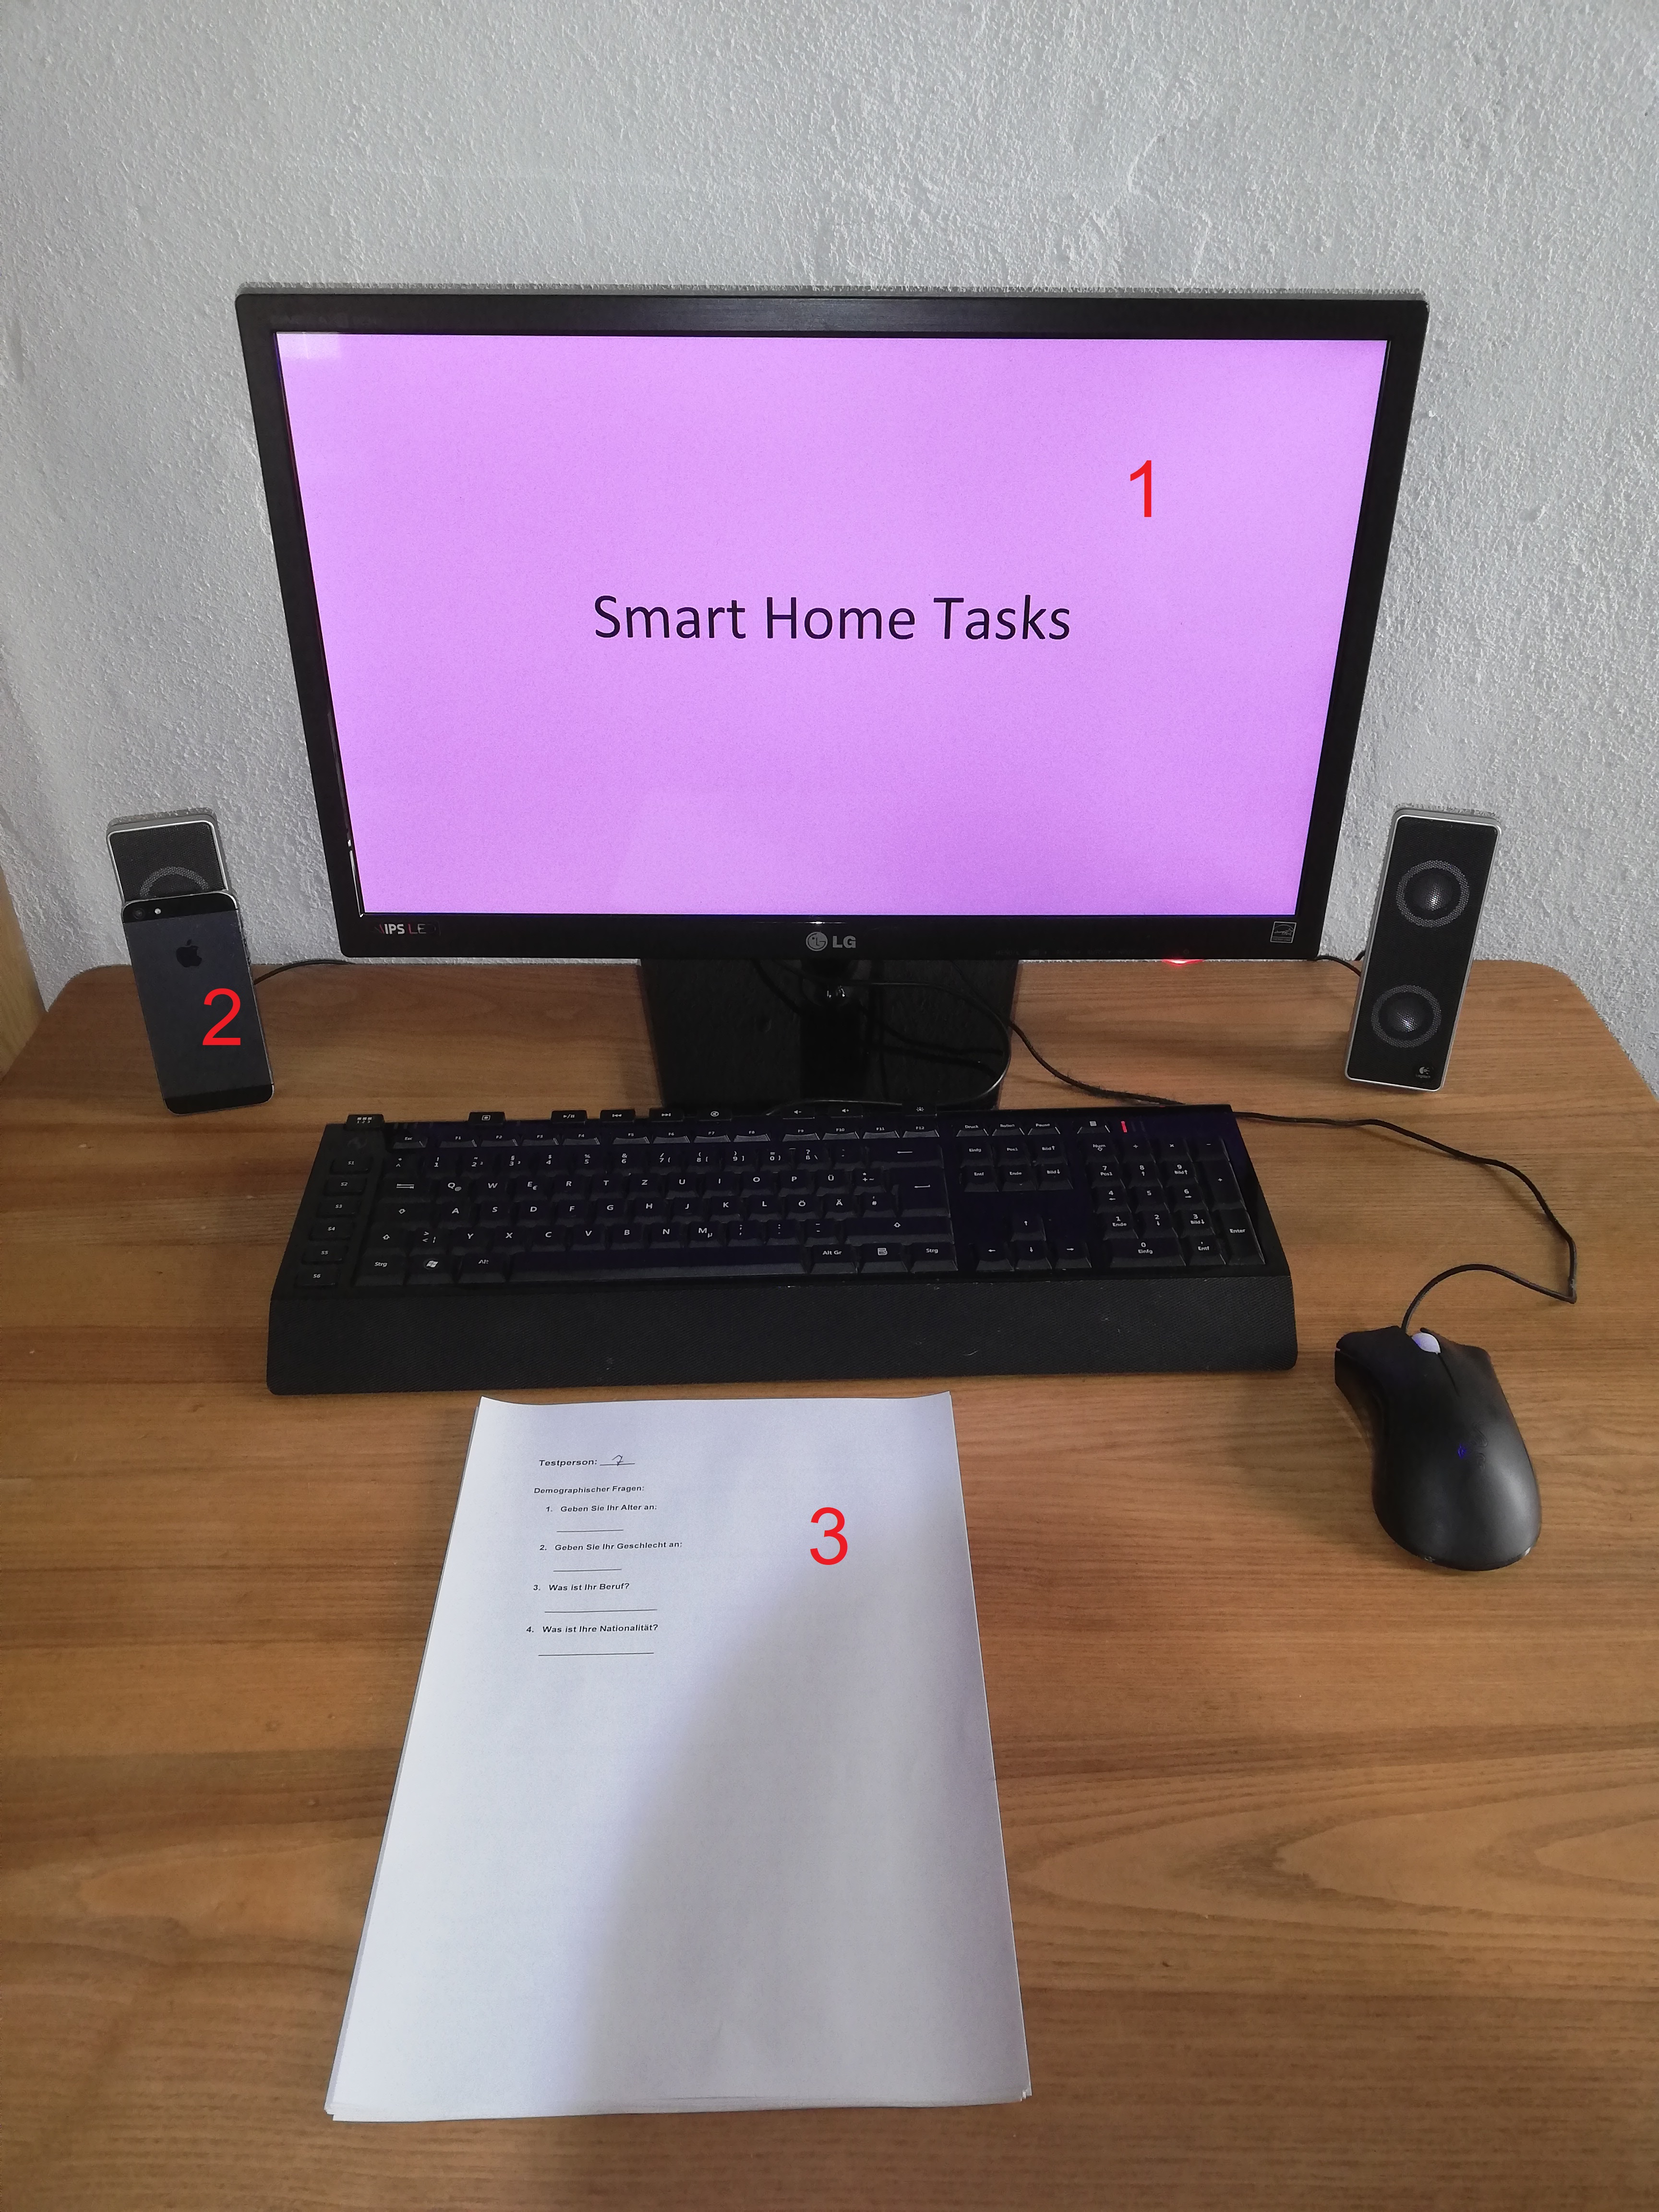
\includegraphics[width=\columnwidth]{SetupZahlen}
		\caption{Setup with monitor to illustrate smart home tasks (1), camera for video recording (2) and the questionnaires (3)}
		\label{figure:Setup}
		\Description{Setup with monitor to illustrate smart home tasks (1), camera for video recording (2) and the questionnaires (3)}
	\end{figure}
	
	\subsection{Procedure}
	Before starting the session, the participants were asked to fill out a consent form and a demographic questionnaire. Then they had to fill out a questionnaire in terms of their previous knowledge and usage of smart home devices and the three interaction modalities. After that the tasks were presented to the participants in a random order. At first all tasks had to be fulfilled with a single interaction modality, then with the second and after that with the remaining modality. Additionally to the illustration through pictures, the tasks were explained verbally. The participants were allowed to talk, move and interact with a display in any way they wanted and were encouraged to explain their choices in a thinking-aloud approach. After each task the participants rated their specific suggestion on goodness, ease, enjoyment and social acceptance on four 7-point Likert scales. 
	
	When all tasks were finished with each interaction modality the participants rated the three interaction modalities for each on 7-point Likert scales, on how good each modality is to perform the specific task. They were asked to do this independently of their own suggestions. At the end a semi-structured interview was conducted to explore the motivation of the participants for each choice and allow them to rate the different interaction modalities under the aspects of efficiency, simplicity, naturality, desirability and enjoyment. this is based on a similar approach in the elicitation study on foot gestures by Felberbaum et al. \cite{Felberbaum.2018}. The study took about an hour, for which the participants were compensated with sweets.
	
	\section{Results}
	With nine participants and eleven tasks, we collected for each of the three interaction modalities $143$ suggestions and in total $13*11*3=429$. Our results include the video recording, taxonomies for each interaction modality, user-defined sets of voice commands, display interactions and gestures, subjective ratings of the sets, qualitative observations and an assessment on the modalities for each task. 
	
	\subsection{Classification of Voice Commands}
	The participants suggested $43$ unique voice commands. The authors manually classified each voice command along five dimensions: \textit{nature}, \textit{form}, \textit{flow}, \textit{context} and \textit{complexity}. Within each dimension are multiple categories, shown in Table \ref{tab:taxVoice}. We adopted the dimensions from Wobbrock \textit{et al.} \citep{Wobbrock.2009} and Ruiz \textit{et al.} \citep{Ruiz.2011} and adapted them to voice commands. 
	
	\subsubsection{Taxonomy of Voice Commands}
	The \textit{nature} dimension comprises \textit{action} voice commands which state the action to perform. An example of this type of voice command is saying "increase temperature". \textit{State} voice commands describe the desired condition of a device. For example, a \textit{state} voice command is "cameras on" to start camera surveillance.
	
	The \textit{form} dimension describes how much words are used in the voice command and if they have the structure of a full sentence. A \textit{single word} command can be "next" to get to the next TV channel. \textit{Two words} voice commands mostly consist out of the mentioning of the device to be controlled and an action or state. \textit{More words} commands are similar to \textit{two words} but use additional filler words. Finally, voice commands that are correct sentences were classified with the category \textit{sentence}.
	
	The \textit{flow} dimension categorizes the voice commands, if response of a device occurs after or while the user acts. A voice command is\textit{discrete}, when a device performs the command after the participant stopped talking. A \textit{continuous} voice command would be starting an action with a command and stop the ongoing action with another command.
	
	The \textit{context} dimension describes, if the voice command requires a specific context or can be performed independently. For example saying "turn off" to turn off the oven is \textit{in-context}, whereas "oven off" is considered \textit{no-context}.
	
	The \textit{complexity} dimension describes if the voice command consists out of a single or a composition of more voice commands. A \textit{compound} voice command can be decomposed into \textit{simple} voice commands.
	\begin{table}[t]
		\begin{center}
			\caption{Taxonomy of voice commands for smart home tasks}
			\label{tab:taxVoice}
			\begin{footnotesize}
				\begin{tabular}{p{0.2\columnwidth} p{0.2\columnwidth} p{0.5\columnwidth}} \toprule
					\multicolumn{3}{c}{\textit{Taxonomy of voice commands}} \\ \midrule
					\textbf{Nature}		& Action		& Voice command states the action to perform \\
										& State			& Voice command describes the desired condition \\ \midrule
					\textbf{Form} 		& Single word	& Voice command consists out of a single word \\
										& Two words		& Voice command consists out of two words \\
										& More words	& Voice command consists out of more words without sentence structure \\
										& Sentence		& Voice command uses sentence structure \\ \midrule
					\textbf{Flow}		& Discrete		& Response occurs \textit{after} the user acts \\ 
										& Continuous 	& Response occurs \textit{while} the user acts  \\ \midrule
					\textbf{Context}	& In-context	& Voice command requires specific context \\
										& No-context	& Voice command does not require specific context \\ \midrule
					\textbf{Complexity}	& Simple		& Voice command consists of a single voice command \\
										& Compound		& Voice command can be decomposed into simple voice commands  \\ \bottomrule
				\end{tabular}
			\end{footnotesize}
		\end{center}
	\end{table}
	\subsection{User-defined Voice Commands}
We collected a total of $143$ voice commands, which we used to create a user-defined voice command set for the 11 tasks. For each task, we grouped identical voice commands together and the group with largest size was chosen to be the representative voice command for this corresponding task. To evaluate the degree of consensus among the participants, we computed the \textit{agreement score} $A_t$ (Equation \ref{eq:agreement score}), as proposed by Vatavu and Wobbrock \cite{Vatavu.2015}, for each task.
		\begin{equation}
			\label{eq:agreement score}
			A_t = \frac{|P_t|}{|P_t|-1} \sum_{P_i \subseteq P_t} \left(\frac{|P_i|}{|P_t|}\right)^2  - \frac{1}{|P_t|-1}
		\end{equation}
In equation \ref{eq:agreement score}, $t$ is a task in the set of all tasks $T$, $P_t$ is the set of suggested voice commands for $t$ and $P_i$ is a subset of identical voice commands from $P_t$. 
As an example of calculation of an agreement score, consider the task \textit{increase the volume of the music}. The task has four groups of identical voice commands with a size of $7$, $4$, $1$ and $1$. Therefore the agreement score for \textit{increase the volume of the music} is:
		\begin{equation}
			A = \frac{13}{12} \left(\left(\frac{7}{13}\right)^2 + \left(\frac{4}{13}\right)^2 + \left(\frac{1}{13}\right)^2 + \left(\frac{1}{13}\right)^2 \right)- \frac{1}{12} = 0.346
		\end{equation}
		Figure \ref{figure:ASall} illustrates the agreement scores for each task (voice commands: green). Participants had the least agreement on commands for the tasks \textit{start multi-colored wash at 60 degree} (Task 3) and \textit{increase the room temperature} (Task 5). This is attributable to the complexity of the tasks.
		\begin{figure*}			
			\centering
			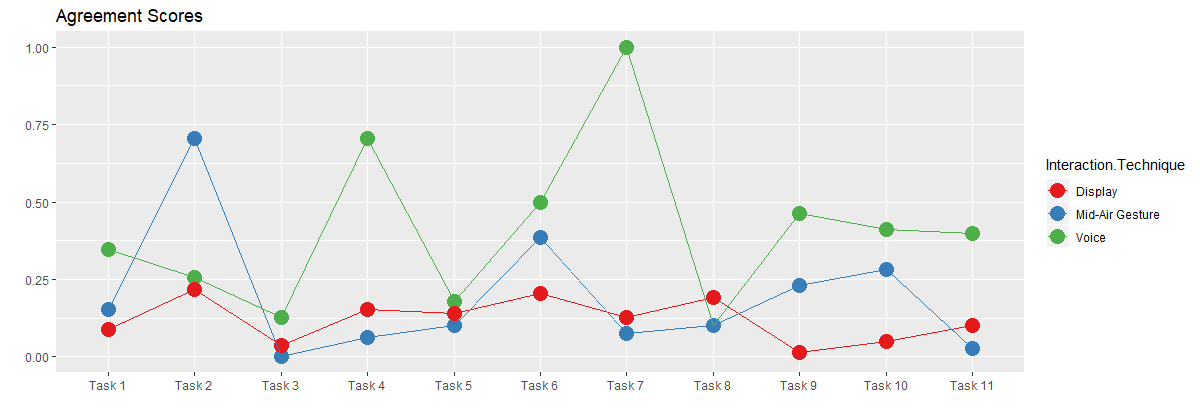
\includegraphics[width=\textwidth]{AgreementScoresAllTechniques}
			\caption{Agreement scores for each task with of all interaction modalities}
			\label{figure:ASall}
			\Description{Agreement scores for each task with of all interaction modalities}
		\end{figure*}
%		\begin{figure*}			
%			\centering
%			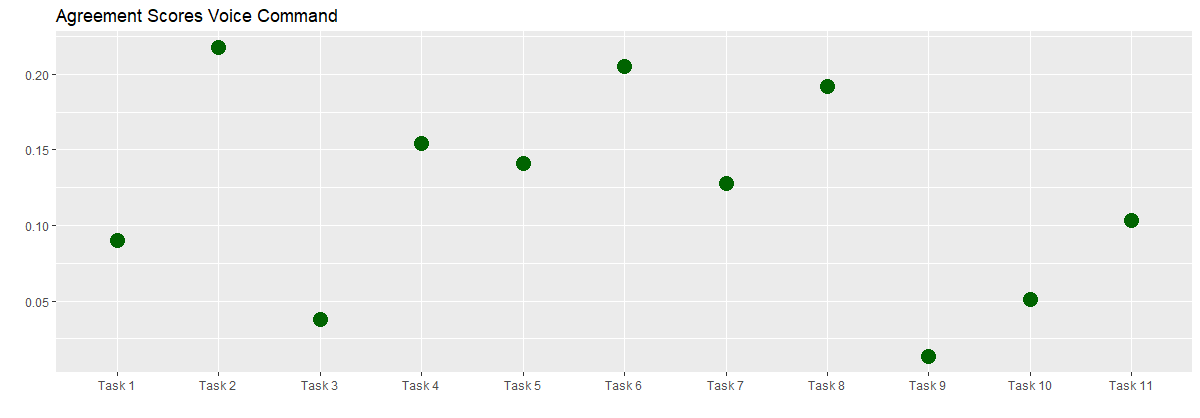
\includegraphics[width=\textwidth]{AgreementVoice}
%			\caption{Agreement scores for each task with voice commands}
%			\label{figure:ASvoice}
%			\Description{Agreement scores for each task with voice commands}
%		\end{figure*}
	Since the study was conducted in German, we also provide the original version of the voice commands to prevent losses during translation. Table \ref{tab:UserVoice} shows the most common and second most common voice commands and their frequency according to the different tasks.
	\begin{table}[t]
		\begin{center}
			\caption{User defined voice command set with the two most common options for each task}
			\label{tab:UserVoice}
			\begin{footnotesize}				
				\begin{tabular}{p{0.07\columnwidth} p{0.3\columnwidth} p{0.3\columnwidth} R{0.16\columnwidth}} \toprule
					\textbf{Task}	& \textbf{German}			& \textbf{English}		& \textbf{Frequency} \\ \midrule
					1				& lauter					& louder				& 53.8 \% \\ 
									& Musik lauter				& music louder			& 30.8 \% \\ \midrule
					2				& N\"achster Kanal			& next channel			& 46.2 \% \\
									& weiter					& next					& 23.1 \% \\ \midrule
					3				& Buntw\"asche 60 Grad			& colored laundry 60 degrees		& 30.8 \% \\ 
									& Starte Buntw\"asche 60 Grad	& start colored laundry 60 degrees	& 15.4 \% \\ \midrule
					4				& Ofen aus					& oven off				& 84.6 \% \\
									& ausschalten				& turn off				&  7.7 \% \\ \midrule
					5				& W\"armer					& warmer					& 30.8 \% \\
									& Raumtemperatur erh\"ohen	& increase room temperature	& 30.8 \% \\ \midrule
					6				& Rollladen \"offnen		& open roller shutter	& 69.2 \% \\
									& Rollladen auf				& roller shutter up		& 23.1 \% \\ \midrule
					7				& Licht an 					& light on 				& 100.0 \% \\ \midrule
					8				& Licht dimmen				& dim light				& 30.8 \% \\
									& Licht dunkler				& light darker			& 15.4 \% \\ \midrule
					9				& Fenster schlie{\ss}en		& close window			& 53.8 \% \\
									& Fenster zu				& window closed			& 46.2 \% \\ \midrule
					10				& Haust\"ur absperren		& lock front door		& 61.5 \% \\ 
									& T\"ur zu					& door closed			& 23.1 \% \\ \midrule
					11				& Kamera an					& camera on				& 61.5 \% \\ 
									& Kamera einschalten		& switch on camera		& 23.1 \% \\ \bottomrule
				\end{tabular}
			\end{footnotesize}	
		\end{center}
	\end{table}	
	\subsection{Classification of Display Interactions}
	The participants suggested $61$ unique display interactions. Similar to the voice commands we manually classified each display interaction along three dimensions for \ac{gui} elements (\textit{form}, \textit{elements}, \textit{flow}) and for touch gestures along four dimensions (\textit{form}, \textit{nature}, \textit{binding}, \textit{flow}). Within each dimension are multiple categories, shown in Table \ref{tab:taxDisplayGUI} for \ac{gui} elements and for touch gestures in Table \ref{tab:taxDisplayTG}. The dimensions and categories for \ac{gui} elements were inspired by the work from Wobbrock \textit{et al.} \citep{Wobbrock.2009} and Ruiz \textit{et al.} \citep{Ruiz.2011}. As taxonomy for touch gestures we used Wobbrock \textit{et al.} \citep{Wobbrock.2009} taxonomy of surface gestures, witch is displayed in Table \ref{tab:taxDisplayTG}.
	\subsubsection{Taxonomy of Display Interaction (\ac{gui} Elements):}
	The \textit{form} dimension describes, if the display interaction consists of a single action that leads to a response or if it consists of a selection of a desired action that is started through another element. A \textit{direct action} would be a single click on a button to turn the light on. Selecting a washing program and starting it with an additional "Start"-Button would be considered \textit{selection \& confirmation}.
	
	The \textit{elements} dimension describes, what kind of \ac{gui} elements where used for the display interaction. \textit{Single clickables} are elements which emit a response after a single click, like buttons or checkboxes. The category \textit{slider} is chosen, when one or more sliders are included in the \ac{gui}, for example to change the volume of music. Rotational elements like the selection of washing programs with the representation of a rotary knob is categorised as \textit{rotation}. \textit{Text \& number entry} includes options to enter something with a keyboard. Special symbolic elements, like dragging wood into a fire, to increase the room temperature are considered \textit{symbolic}.
	
	The \textit{flow} dimension again categorizes this time the display interactions, if response of a device occurs after or while the user acts. A \textit{descrete} display interaction would be, pressing a "Close Window" button and after that the command is executed. A \textit{continuous} one would be, dragging the regulator on a slider to adjust the volume of music simultaneously.
	\begin{table}[t]
		\begin{center}
			\caption{Taxonomy of display interactions for smart home tasks (\ac{gui} elements)}
			\label{tab:taxDisplayGUI}
			\begin{footnotesize}				
				\begin{tabular}{p{0.2\columnwidth} p{0.2\columnwidth} p{0.5\columnwidth}} \toprule
					\multicolumn{3}{c}{\textit{Taxonomy of display interactions (\ac{gui} elements)}} \\ \midrule
					\textbf{Form}		& Direct Action				& Single interaction that directly leads to the action \\
										& Selection \& Confirmation	& Selection of the action and starting through another element\\ \midrule
					\textbf{Elements} 	& Single clickables			& The \ac{gui} includes one or more single clickables 
																	  (button, checkbox, etc.) \\
										& Slider					& The \ac{gui} includes one or more sliders \\
										& Rotation					& The \ac{gui} includes one or more rotational elements \\ 
										& Text \& number entry		& The \ac{gui} includes one or more options to enter text or numbers \\
										& Symbolic					& The \ac{gui} includes one or more special symbolic elements\\ \midrule
					\textbf{Flow}		& Discrete					& Response occurs \textit{after} the user acts \\ 
										& Continuous 				& Response occurs \textit{while} the user acts  \\ \bottomrule
				\end{tabular}
			\end{footnotesize}	
		\end{center}
	\end{table}	
	\subsubsection{Taxonomy of Display Interaction (Touch Gestures):}	
	As stated before we adopted the taxonomy of surface gestures from Wobbrock \textit{et al.} \citep{Wobbrock.2009} for our taxonomy of display interaction (touch gestures). (ToDo/Frage: Muss diese dann auch wie die anderen beschrieben werden?)
	\begin{table}[t]
		\begin{center}
			\caption{Taxonomy of display interactions for smart home tasks (touch gestures)}
			\label{tab:taxDisplayTG}
			\begin{footnotesize}
				\begin{tabular}{p{0.12\columnwidth} p{0.28\columnwidth} p{0.5\columnwidth}} \toprule
					\multicolumn{3}{c}{\textit{Taxonomy of display interactions (touch gestures)}} \\ \midrule
					\textbf{Nature}		& Symbolic				& Gesture visually depicts a symbol \\
										& Physical				& Gesture acts physically on objects \\ 
										& Metaphorical 			& Gesture indicates a metaphor \\ 
										& Abstract				& Gesture-referent mapping is arbitrary \\ \midrule
					\textbf{Form} 		& Static pose			& Hand pose is held in one location \\
										& Dynamic pose			& Hand pose changes in one location \\
										& Static pose and path 	& Hand pose is held as hand moves \\
										& Dynamic pose and path	& Hand pose changes as hand moves \\
										& One-point touch		& Static pose with one finger \\ 
										& One-point path		& Static pose and path with one Finger \\ \midrule
					\textbf{Binding}	& Object-centric 		& Location defined with respect to object features \\
										& World-dependent 		& Location defined with respect to world features \\
										& World-independent 	& Location can ignore world features \\
										& Mixed dependencies	& World-independent plus another \\ \midrule
					\textbf{Flow}		& Discrete				& Response occurs \textit{after} the user acts \\ 
										& Continuous 			& Response occurs \textit{while} the user acts  \\ \bottomrule
				\end{tabular}
			\end{footnotesize}
		\end{center}
	\end{table}
	\subsection{User-Defined Display Interactions}
	We collected also $143$ display interactions, which we once again sorted into groups of identical display interactions. The group with the largest size was chosen as the representative display interaction for the corresponding task. The \textit{agreement score} (Equation \ref{eq:agreement score}) was calculated for each task to evaluate the degree of consensus among the participants. They are shown in Figure \ref{figure:ASall} (red). The overall low \textit{agreement scores} can be explained by the big amount of different \ac{gui} elements and touch gestures. 
	Table \ref{tab:UserDisplay} shows the most common and second most common display interaction and their frequency according to the different tasks.
	\begin{table}[t]
		\begin{center}
			\caption{User defined display interaction set with the two most common options for each task}
			\label{tab:UserDisplay}
			\begin{footnotesize}				
				\begin{tabular}{p{0.07\columnwidth} p{0.6\columnwidth} R{0.16\columnwidth}} \toprule
					\textbf{Task}	& \textbf{Display Interaction}				& \textbf{Frequency} \\ \midrule
					1				& vertical slider							& 23.1 \% \\ 
									& horizontal slider							& 23.1 \% \\ \midrule
					2				& button with arrow	to the right			& 46.2 \% \\
									& horizontal swipe							& 15.4 \% \\ \midrule
					3				& button with washing program + button with 60 degree		& 23.1 \% \\ 
									& (all others)								&  7.7 \% \\ \midrule
					4				& button with "off"							& 38.5 \% \\
									& vertical slider							& 15.4 \% \\ \midrule
					5				& vertical slider							& 30.8 \% \\
									& button with arrow	to the top				& 23.1 \% \\ \midrule
					6				& button with arrow to the top				& 46.2 \% \\
									& horizontal slider							& 15.4 \% \\ \midrule
					7				& button with "on/off" symbol				& 38.5 \% \\ 
									& button with "on"							& 23.1 \% \\ \midrule
					8				& vertical slider							& 46.2 \% \\
									& (all others)								&  7.7 \% \\ \midrule
					9				& button with window and "close"			& 23.1 \% \\
									& button "close window"						& 23.1 \% \\ \midrule
					10				& button with lock							& 23.1 \% \\ 
									& button with key							& 15.4 \% \\ \midrule
					11				& button with camera						& 30.8 \% \\ 
									& button with "on/off" symbol				& 15.4 \% \\ \bottomrule
				\end{tabular}
			\end{footnotesize}	
		\end{center}
	\end{table}	
	\subsection{Classification of Mid-Air Gestures}
	The participants suggested $55$ unique mid-air gestures. Once again we manually classified each mid-air gesture, this time along eight dimensions. The dimensions are \textit{nature}, \textit{flow}, \textit{context}, \textit{interaction}, \textit{dimension}, \textit{position}, \textit{movement} and \textit{complexity}. Within each dimension are multiple categories, shown in Table \ref{tab:taxGestures}. We adopted the dimensions \textit{nature} (small adjustment at category \textit{physical}), \textit{flow}, \textit{context} and \textit{complexity} and their corresponding categories from Wobbrock \textit{et al.} \citep{Wobbrock.2009} and Ruiz \textit{et al.} \citep{Ruiz.2011}. \textit{Dimension} from Ruiz \textit{et al.} \citep{Ruiz.2011} was adapted to our needs. \textit{Interaction} was inspired by Dingler \textit{et al.} \citep{Dingler.2018} and we further extended the taxonomy by the two dimensions \textit{position} and \textit{movement}.
	\subsubsection{Taxonomy of Mid-Air Gestures:}
	The \textit{nature} dimension includes \textit{symbolic} mid-air gestures, which visually depict symbols. An example for that is drawing a "X" into the air to turn off the oven. \textit{Physical} mid-air gestures imitate real physical actions like locking a door with a key, by rotating the wrist with a fist like hand position. A \textit{metaphorical} gesture may be wrapping the arms around yourself with rubbing, to indicate you are freezing and want to raise the temperature in the room. Mid-air gestures that did not fit into any of these three categories are classified as \textit{abstract}.
	
	The \textit{flow} dimension is the same as in the other taxonomies and categorizes the mid-air gestures, if response of a device occurs after or while the user acts. A mid-air gesture is\textit{discrete}, when the response occurs after the movement, and \textit{continuous}, when the response occurs during the movement. 
	
	The \textit{context} dimension describes, if the mid-air gesture requires a specific context or can be performed independently. For example making a horizontal hand movement to change the TV channel is \textit{in-context}, whereas pointing at the TV and then performing the hand movement is considered \textit{no-context}.
	
	The \textit{interaction} dimension simply describes if the participant used only one hand or both hands for their suggested mid-air gesture.
	
	The \textit{dimension} of a mid-air gesture is used to describe how many axis are involved in the movement of the hand. Some gestures, like just rotating the wrist happen along only a single axis. The translation of a hand or a rotational motion from the wrist are considered \textit{tri-axis}. The combination of those two movements is classified as \textit{six-axis}. The movement of fingers was ignored in this dimension and is described more in the dimension \textit{movement}.
	
	The \textit{position} dimension describes the finger position at the beginning of the mid-air gesture. The difference between \textit{flat hand} and \textit{open hand} is, that the fingers are together at \textit{flat hand} and spread at \textit{open hand}.
	
	The \textit{movement} dimension simply states if the participant includes relevant finger movement (\textit{movement}) or no finger movement (\textit{no movement}) into his mid-air gesture. 
	
	The \textit{complexity} dimension describes, just like voice commands, if the mid-air gesture consists out of a single or a composition of more mid-air gestures. A \textit{compound} mid-air gesture can be decomposed into \textit{simple} gestures.	
	\begin{table}[t]
		\begin{center}
			\caption{Taxonomy of mid-air gestures for smart home tasks}
			\label{tab:taxGestures}
			\begin{footnotesize}
				\begin{tabular}{p{0.15\columnwidth} p{0.2\columnwidth} p{0.5\columnwidth}} \toprule
					\multicolumn{3}{c}{\textit{Taxonomy of mid-air gestures for smart home tasks}} \\ \midrule
					\textbf{Nature}		& Symbolic			& Gesture visually depicts a symbol \\
										& Physical			& Gesture imitates a physical action \\ 
										& Metaphorical 		& Gesture indicates a metaphor \\ 
										& Abstract			& Gesture-referent mapping is arbitrary \\ \midrule
					\textbf{Flow}		& Discrete			& Response occurs \textit{after} the user acts \\ 
										& Continuous 		& Response occurs \textit{while} the user acts  \\ 
					\textbf{Context}	& In-context		& Gesture requires specific context \\
										& No-context		& Gesture does not require specific context \\ \midrule
					\textbf{Interaction}& One hand			& Gesture was performed with one hand \\
										& Two hands			& Gesture was performed with two hands \\ \midrule
					\textbf{Dimension}	& Single-Axis		& Motion occurs around a single axis from \\
										& Tri-Axis			& Motion involves either translational motion from hand or rotational motion from wrist, not both \\
										& Six-Axis			& Motion involves translational motion from hand and rotational motion from wrist \\ \midrule
					\textbf{Position}	& Flat hand			& Gesture started with flat hand \\
										& Open hand			& Gesture started with open hand \\
										& Closed hand		& Gesture started with closed hand (fist) \\
										& Single finger		& Gesture started with a single outstretched finger \\
										& Two fingers		& Gesture started with two outstretched fingers \\
										& More fingers		& Gesture started with three or four outstretched fingers \\ \midrule
					\textbf{Movement}	& No movement		& No change in finger position \\
										& Movement			& Change in finger position \\ \midrule
					\textbf{Complexity}	& Simple			& Gesture consists of a single gesture \\
										& Compound			& Gesture can be decomposed into simple gestures \\ \bottomrule
				\end{tabular}
			\end{footnotesize}
		\end{center}
	\end{table}
	\subsection{User-Defined Mid-Air Gestures}
	We collected $142$ mid-air gestures, because one participant could not think of a mid-air gesture for starting the  multi-colored wash at $60$ degree. Then we followed the procedure as with voice commands and display interactions. We grouped the identical mid-air gestures together, chose the group with the largest size as representative gesture for the corresponding task and computed the \textit{agreement score} (Equation \ref{eq:agreement score}) for each task. The latter are also shown in Figure \ref{figure:ASall} (blue). Task 3 (\textit{start multi-colored wash at 60 degree}) has an \textit{agreement score} of $0.0$ because there were no two identical mid-air gestures. Compared to the other two modalities the participants had the highest agreement on Task 2 (\textit{turn on the next TV channel}) with an \textit{agreement score} of $0.705$. Table \ref{tab:UserGesture} shows the two most common mid-air gestures for each task with their frequency.
%	\begin{figure*}			
%		\centering
%		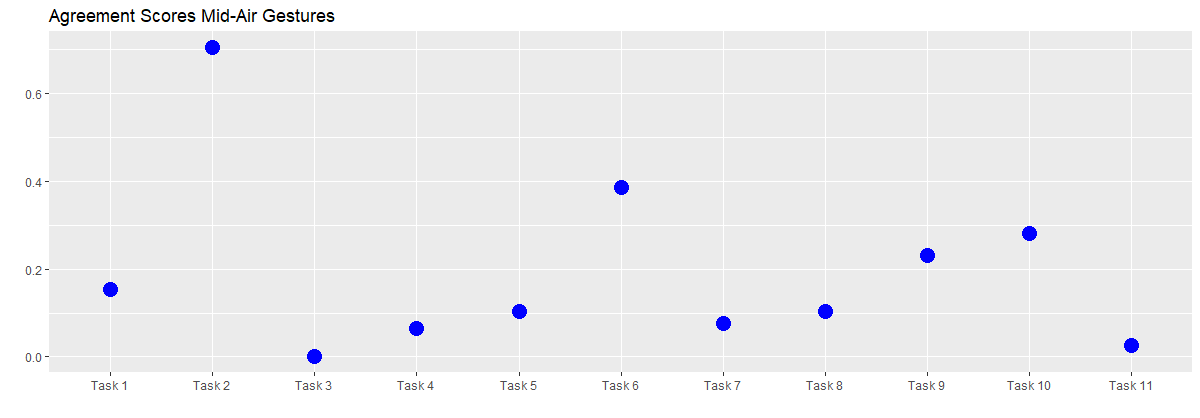
\includegraphics[width=\textwidth]{AgreementGesten}
%		\caption{Agreement scores for each task with mid-air gestures}
%		\label{figure:ASgesture}
%		\Description{Agreement scores for each task with mid-air gestures}
%	\end{figure*}
	\begin{table}[t]
		\begin{center}
			\caption{User defined mid-air gesture set with the two most common options for each task}
			\label{tab:UserGesture}
			\begin{footnotesize}				
				\begin{tabular}{p{0.07\columnwidth} p{0.6\columnwidth} R{0.16\columnwidth}} \toprule
					\textbf{Task}	& \textbf{Display Interaction}				& \textbf{Frequency} \\ \midrule
					1				& one hand, vertical motion 				& 38.5 \% \\ 
									& one hand, hand rotation					& 15.4 \% \\ \midrule
					2				& one hand, horizontal motion				& 84.6 \% \\
									& (the two others)							&  7.7 \% \\ \midrule
					3				& (all different)							&  7.7 \% \\ \midrule 
					4				& one hand, horizontal motion				& 23.1 \% \\ 
									& both hands, cross in front of body 		& 15.4 \% \\ \midrule
					5				& one hand, vertical motion					& 23.1 \% \\
									& one hand, thump up, vertical motion		& 23.1 \% \\ \midrule
					6				& one hand, vertical motion					& 61.5 \% \\
									& both hands, vertical motion				& 15.4 \% \\ \midrule
					7				& one hand, flicking with the finger		& 23.1 \% \\ 
									& one hand, open closed hand				& 15.4 \% \\ \midrule
					8				& one hand, vertical motion					& 30.8 \% \\
									& one hand, hand rotation					& 15.4 \% \\ \midrule
					9				& one hand, hand rotation					& 38.5 \% \\
									& one hand, pushing motion					& 30.8 \% \\ \midrule
					10				& one hand, hand rotation					& 53.8 \% \\ 
									& both hands, bring together from outside in front of the body	& 15.4 \% \\ \midrule
					11				& one hand, open closed hand				& 15.4 \% \\ 
									& one hand, vertical motion					& 15.4 \% \\ \bottomrule
				\end{tabular}
			\end{footnotesize}	
		\end{center}
	\end{table}	
	
	\subsection{Comparing the Modalities}
	
	The three modalities shall be compared now.
	
	Home entertainment (Task 1: Increase the volume of the music and Task 2: Turn on the next tv channel). In Task 1 the participants preferred display and voice control, which were very close to each other. The mean of the voice-rating was 5.625 and the mean of the display-rating was 5.692. In task 2 they preferred display and rated it with 6.385. This task is the only one, in which gesture control was not the most unpopular method. In this case gesture control was rated with 5.077 while voice control was rated with 4,846.
	
	For the category smart household appliances (Task 3: Start multi-colored wash at 60 degree  and task 4: Turn off the oven), the participants preferred display- and voice-techniques. In task 3 with 6.231 the display was rated better than voice-control with 5.154, while they assessed gestures bad (1.462). In task 4 the difference between voice (5.923) and display(6.231) was less than in Task 3, but the participants still preferred display control. Also in this task, the gestures with 3.077 were less popular than the other methods.
	
	For the Energy Management category(Task 5: Increase the room temperature and Task 6: Open the shutters), the participants prefer display and voice techniques too. In task number 5 the participants preferred display interaction (6.154) before voice-interaction (5.923), in task number 6 they preferred voice (6.231) instead of display (5.692). In both tasks, the gestures were rated worse than the other methods. In task 5 the score is 3.308 in task 6 the gesture score is 5.077.
	
	In the Comfort and light category, (Task 7: Turn on the light and Task 8: Dim the light) for task number 7 they preferred voice (6.077) before display (5.692) and gestures (5.154) in task number 8 display (6.154) before voice (5.231) and gestures (4.308). 
	
	In the building security category, the relation of the methods in the single tasks is very similar to the relations of the other tasks. In Task 9, the score of the display control is 6.385 while the score of voice control is 6.308 and the score of gesture control is 3.923. In Task 10 the score of the display control is 5.615, the score of voice control is 5.462 and the score of the gesture control is 3.769. In Task 11, the display score is 6.231, the voice score is 6.154 and the gesture score is 3.231. Display and voice are rated very similar, while gestures are less liked.
	All the values a visualized in Figure \ref{figure:ModalityRating}.
	\begin{figure}			
		\centering
		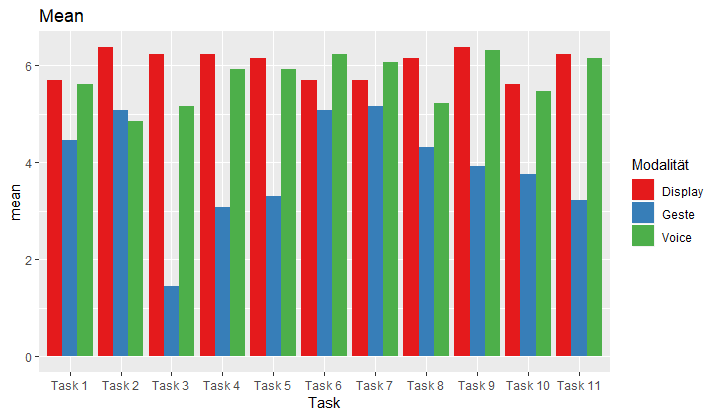
\includegraphics[width=\columnwidth]{MeanGesamt}
		\caption{Modalities rated by the participants, for each task on a scale from 1="not fitting at all" to 7="very fitting"}
		\label{figure:ModalityRating}
		\Description{Modalities rated by the participants, for each task on a scale from 1="not fitting at all" to 7="very fitting"}
	\end{figure}
	
	\subsection{Qualitative Results}
	The qualitative data obtained through the semi-structured interview was analysed by splitting the participants opinions into six categories, obtained through an open-coding approach carried out by the three researchers individually. These are evaluation of the experiment, voice control, display control and mid-air gesture control, as well as possible mixtures of interaction modalities and further suggested ones. 
	
	The participants mainly thought of the experiment as interesting and innovative. Participants stated it was "entertaining and interesting to test out new things I've never done before". 
	
	Looking into general opinions on the different interaction modalities, the participants voice mainly favourable opinions about voice control. They stated voice control is "clear and unambiguous, like commanding". Display control was regarded as easy to control and intuitive, "it's the most universal and comfortable to use", while also classing it as time-consuming, stating it's "tedious, always having to hold a display, like a smart phone, in your hands". On the other hand, participants were not as convinced by mid-air gesture control, as is mirrored in the collected quantitative data. They stated it's "complicated to use" and "only intuitive if all gestures are the same", explaining that "gestures you use seldom, you completely forget after like a month". The surveillance aspect also valued into those opinions, with participants stating that "I don't want to be under constant surveillance, I wouldn't implement such an interaction technique", which also influenced their view on voice control, even though not as much, as participants specified that "voice control is not as bad as video monitoring, though it would be better if you could turn it off.". 
	
	When asked about the possibilities of mixing two or three of the suggested interaction modalities in one smart home environment, participants were generally in favour of it, stating "combining like two, like voice and display, would be the most convenient". Participants were also asked about other interaction modalities different from voice, gesture and display control that come to their mind, resulting in interesting approaches for possible future work such as "I'd like haptic feedback, such as stomping once on the floor to activate my underfloor heating" or "I don't want to talk too much to my smart home, I want it to know my demands autonomously". 
	
	\section{Discussion}
	The paper deals with the question, what interaction modality fits best. To find out about this, quantitative and qualitative data were compiled.  We found out that participants prefer to use voice commands and display interactions in all categories except of category 1. In Task 2 participants would rather use mid-air gestures instead of voice commands. Still, they prefer to use display control.
	Table \ref{tab:AllModalitiesRating} clarifies this.
	\begin{table}[h]
		\begin{center}
			\caption{Ratings of the modalities across all tasks}
			\label{tab:AllModalitiesRating}
			\begin{footnotesize}				
				\begin{tabular}{p{0.2\columnwidth} R{0.2\columnwidth} R{0.2\columnwidth}} \toprule
								& \textbf{Mean}		& \textbf{STD} \\ \midrule
					Voice		& 5.720				& 1.350 \\ \midrule
					Display		& 6.042				& 1.368 \\ \midrule
					Gestures	& 3.895				& 1.901  \\ \bottomrule
				\end{tabular}
			\end{footnotesize}	
		\end{center}
	\end{table}		
	It is necessary to look deeper into the data to interpret this table. Therefore the results from the three interaction modalities shall be examined.
	
	It can be seen, that the voice commands were rated best in goodness, while display interaction was rated second best. The participants explained that for them voice control was clear and like commanding. This supports the fact that voice was rated best for goodness. The display interaction was rated best in ease, voice commands were rated second best. The participants described the display interaction as easy to control and comfortable to use. Furthermore they are already familiar with this kind of interaction. 
	
	It seems, the ease of use made the participants feel less awkward, with 1.182, display control reached the best social accept score of all methods. 
	
	The enjoyment was the highest when the participants used display control and second highest, when they used voice-commands. 
	
	Both tables show that voice and display are rated very similar. The qualitative data from the interviews supports this. 
	
	The participants told, that gestures were complicated and impractical. It can be seen that especially the tasks which need awkward gestures are rated bad. The dislike of mid -air gestures was lower in tasks which need only simple gestures, like task 1, 2, 6, 7. 
	
	Most of the users could imagine to use more than one method. Most of them preferred a mix or a choice of voice commands and display interaction, depending on the task.
	
	Independent of the single tasks the surveillance aspect influenced the participants. It seemed, that the video monitoring alienated the participants more than the voice recording. This of course affected the choice of methods.
	
	The choice of what method is the most popular depends on the task. The participants preferred simple and functional usage. Because of that participants wish to use voice control or display control. Gesture control seems only conceivable in simple tasks. Besides it is cumbersome and complicated, the participants felt less comfortable using it. 
	\begin{table}[h]
		\begin{center}
			\caption{Ratings of goodness, ease, enjoiment and social acceptance for the modalities across all tasks}
			\label{tab:AllModalitiesGEES}
			\begin{footnotesize}				
				\begin{tabular}{p{0.3\columnwidth} R{0.15\columnwidth} R{0.15\columnwidth} R{0.15\columnwidth}} \toprule
												& \textbf{Voice}	& \textbf{Display}	& \textbf{Gestures} \\ \midrule
					\textbf{Goodness}			& 6.629				& 6.294 			& 5.380 \\ \midrule
					\textbf{Ease}				& 6.301				& 6.350 			& 5.655 \\ \midrule
					\textbf{Enjoiment}			& 5.049				& 5.231 			& 4.704 \\ \midrule
					\textbf{Social acceptance}	& 1.685				& 1.182				& 2.437 \\ \bottomrule
				\end{tabular}
			\end{footnotesize}	
		\end{center}
	\end{table}

	\section{Future Work}
	Future work can build on the qualitative research that showed participants stating they mostly prefer display and voice control, with a possible combination of these two interaction modalities. Further work needs to focus on this approach, while also testing a combination of interaction modalities within a setting including more actual implemented parts of a smart home system. Although simulations offer research that is faster to develop and perform, they can not guarantee with an absolute certainty users would act the same way in a real smart home environment. 
	The range of the participants was relatively low. Most of them were younger than 30 years old and have a higher education. We only tested German citizens. To achieve a higher transferability and generalizability of the research, it is necessary, to extend the population to draw the participants from. 
	
	Leaving the approach to interact with user's short-time desires leads to us to future work centering around smart home-user interaction for long-time settings. Many of the participants stated their wish to interact with the smart home as little as possible. Instead, they preferred a scenario of setting their needs and demands at an early point in the implementation and rely on the smart home system working autonomous from that moment on. This could lead to a drastic change in participants' viewpoints on goodness, ease and social acceptance of interaction modalities. Performing a command only once compared to multiple times could lead to more lenient opinions on complex voice commands or mid-air gestures, or highly detailed structures of display commands.
	
	Safety issues mentioned in the qualitative research concerning the need to monitor users' in order to implement voice and mid-air gesture control can also lead to further research. In the time of highly demanded data security and privacy, smart homes can not pose as threats to this. Future work can focus on studies developing interaction modalities that are free from such concerns or improve existing modalities to no longer rely on constant user supervision. For this, it's necessary to collaborate with experts of other fields.
	
	\section{Conclusion}
	Our motivation was to find out, if there are some interaction modalities which are more suitable for certain tasks than other modalities. Therefore we conducted a study in which we investigated three smart home interaction modalities, outlining participants preferences for the given tasks on each modality. The particular attention on goodness, ease, enjoyment and social acceptance showed, that there is not a significant difference between the popularity of voice- and display-commands. However there is a significant difference between these methods and mid-air gestures. This can help to understand the advantages and disadvantages of each interaction modality in different areas of smart home assistance. The work also contributes voice, display and mid-air gesture sets based on the most frequently suggested commands for different smart home tasks. The chosen tasks here represented the main fields of smart home assistance. These provided sets can be used as a basis or guideline for researchers developing future voice, display and mid-air gestures or generally smart home based systems. Because voice-commands and display-control were more popular than mid-air gestures, Future work could conzentrate on them.Most of the participants said that they can imagine to use a mixture of both methods. Future work could be to implement such a method. Furthermore future sytems should respect privacy, future work could be to design systems which do not permanent supervice the user.
	
	
	%%
	%% The next two lines define the bibliography style to be used, and
	%% the bibliography file.
	\bibliographystyle{ACM-Reference-Format}
	\bibliography{AUE_Paper}
	
	%%
	%% If your work has an appendix, this is the place to put it.
\end{document}
\endinput
%%
